\section{Methodology}
\label{sec:Methodology}
\subsection{Independent variables}
\subsubsection{Volatility}
In order to keep the amount of data treated at a tractable level\footnote{A quick enquiry returns that the datasets overall more than 20 Gigabytes large, with monthly fund ownership files, segregated into US and international subsamples, being the largest arrays.} and due to data availability limits, stock volatility is measured over a calendar month (end-to-end, adjusted for the number of trading days) as the standard deviation of simple returns using daily close series.

\begin{equation}
  \mathsf{Volatility}_{i, t} = \sqrt{\frac{1}{N\_d_{i, t} - 1} \sum_{d = 1}^{N\_d_{i, t}} (r_{i, d} - \bar{r}_{i, t})^2}
  \end{equation}

Computing and analyzing intraday volatility is a different avenue for research, shown in \textcite{Ben-David2018} : they use the US Trade and Quote (TAQ) database and compute intraday volatility over second-by-second returns, which which is used in a panel OLS regression with the following regressors : the absolute mispricing as a proxy for arbitrage activity, ETF ownership and the same controls included in their monthly database and in this paper (cf. \autoref{subsec:Method:Volatility}, p.\pageref{subsec:Method:Volatility}).
\subsubsection{Liquidity : \textcite{Amihud2002} ratio}
Liquidity has to be implied from various proxy variables. The illiquidity ratio introduced in \textcite{Amihud2002} is one of them and it has been used in literature both as a variable of interest in itself (e.g. \textcite{Israeli2017}) and as a control for the volatility impact of ETF ownership \parencite{Ben-David2018}.

\begin{equation}
  \begin{split}
    \mathsf{Illiq}_{i, t} & = \frac{1}{N\_d_{i, t}} \sum_{d = 1}^{N\_d_{i, t}} \frac{\mid r_{i, d} \mid}{\mathsf{Volume\_D}_{i, d}}\\
    &  = \frac{1}{N\_d_{i, t}} \sum_{d = 1}^{N\_d_{i, t}} \frac{\mid r_{i, d} \mid}{\mathsf{Volume}_{i, d} \cdot \mathsf{VWAP}_{i, d}}
    \end{split}
\end{equation}

  The first line is \textcite{Amihud2002}'s original definition, whereas the second shows that the daily dollar volume, $Volume\_D$, is computed as the product between the volume expressed in terms of stock shares traded, $Volume$, and the volume-weighted adjusted price, or $VWAP$, since it is not an available data in the source database.
  
The method followed in liquidity regressions comes from \textcite{Israeli2017}, which document both liquidity and information-related effects due to ETF ownership : correlation between, on one side, higher ETF ownership  and, on the other side :
\begin{description}
\item[lower liquidity] : higher bid-ask spread and higher price impact of trades
\item[lower price efficiency] : higher stock returns synchronicity, lower future earnings response and, in the long run, lower analyst coverage.
\end{description}

The liquidity regressions will be explained in greater detail in the appropriate subsection (\autoref{subsec:Method:Liquidity}, p.\pageref{subsec:Method:Liquidity}).
\subsubsection{Price efficiency}
\begin{center}
  \textsc{TBD; measures include the forward earnings response coefficient of \textcite{Israeli2017} and the absolute variance ratio of \textcite{Ben-David2018}}
  \end{center}
\subsection{Regressor of interest : ETF ownership}
The purpose of this paper is to identify and quantify the effect of the share of exchange-traded companies' equity being held through ETFs over several characteristics, namely the stocks' volatility, liquidity and price efficiency, all of three will be the dependent variables in dynamic panel regressions. Based on raw monthly fund-stocks number of shares held, the set of funds belonging to the ETF category and the overall number of shares outstanding of the given stock, the percentage of shares outstanding held is determined :
\begin{equation}
  \mathsf{ETF\_Ownership}_{i, t} = \frac{\sum_{f = 1}^{N_{f}} \mathsf{\#\_AdjShares\_Held}_{f, i, t}\cdot B_{f}}{\mathsf{\#\_Shares\_Out}_{i, t}}
\end{equation}
$\forall i = 1:N_{i}$ (stocks), $t = 1:T$ (periods)
with $B_{f} = 1$ if fund $f$ is an ETF, $0$ else.

The reporting frequency plays an important role as far as the accuracy of this variable is concerned: a substantial part of the reporting of their holdings to ETF, which is a regulatory task, is delayed each month : for example, the query for the number of shares owned by an ETF on February 28, 2018 yields a data pointas of the January 31, 2018; the delay can be more than one month. Two competing choices have been tried before it was decided to apply the same rule to the whole sample, out of a need of internal consistency. Even if both branches of this alternative contain disadvantages, a unique choice has to be made regarding the whole sample so that no spurious relationship appears later between one group of stocks and the other. Either unavailable monthly values are considered a marginal share of the aggregate, stock-level ownership ratios, and they are simply ignored, or the latest reported fund-level values are considered the ``best guess'' one can make regarding how many shares of this stock are currently owned through this fund, and they are included in our global, stock-level ratio; this guess will be referred to as \textit{extrapolation}. In other terms, is the bias more severe by including slightly delayed, and therefore possibly outdated portfolios, or by only selecting the information that one has at hand with certainty, though incomplete ? The challenge is to understand, even \textit{a priori}, whether the statistical and even economic interpretation of results will be less hamperedby a main regressor, total ETF ownership, computed precisely wrong (no extrapolation) or approximately correct (short term stale holdings). Without further intuition on the massive data collection and its coverage, one possible way of figuring how serious this issue actually is, is to compare several estimation results obtained with both methodologies. Even if the issue is known, its effects on a large panel are not guaranteed to be sizeable. 

The granular data availability question is also relevant for other institutional ownership controls that will be used to capture a possible influence of other fund types over variables of interest. The fund categories distinguished in the database are, exhaustively, mutual funds, pension funds and hedge funds, all subject to an at least quarterly disclosure of their holdings. Due to the lower update frequency observed with those controls, it has been decided to assume the fund-stock holdings constant between the last available date and the current one, which reduces the volatility of aggregate ownership shares. Another strategy would be to reduce the frequency of observations from monthly to quarterly (at each calendar quarter end) over the whole sample. This estimation strategy remains to investigate in order to state whether such three-month periods are granular enough to perform relevant analyses.
\subsection{Control variables}
\subsubsection{Bid-ask spread}
The most straightforward way to compute the difference between the bid price -- the highest price at which buyers on the market are agreeing to pay for the security on the spot market -- and the ask price -- the lowest price sellers agree to receive for their shares -- is to compute the difference between the variables \texttt{TR.AskPrice} and \texttt{TR.BidPrice} at day close . Whenever both values returned by the data provider are not null, the absolute (difference) measure can be computed and in cross-sectional regressions, the relative measure is used as a liquidity control :
\begin{equation}
  \mathsf{Pct\_BidAskSpread}_{i, t} = \frac{\mathsf{Ask}_{i, t} - \mathsf{Bid}_{i, t}}{\frac{\mathsf{Ask}_{i, t} + \mathsf{Bid}_{i, t}}{2}}
\end{equation}

The denominator in the relative bid-ask spread is the mid-price approximated as the arithmetic average between both quoted prices, without considering the rounding that can occur due to the tick size.

The relative bid-ask spread accounts for the cost of trading, which is itself assumed to correlate positively with the illiquidity, i.e. the weak number of agents willing to trade on a market. The market makers require a higher price, the bid-ask spread, in order to compensate for the risk of note being able to net out their position in an asset rapidly. Thus, a higher bid-ask spread constitutes a limit to arbitrage across markets or assets.

Another explanation has been studied : according to the \textcite{Glosten1985} market-microstructure model, the bid-ask spread reveals the presence of informed traders and it can even exist in a competitive market without trading costs. If there are both informed and uninformed (so-called \emph{noise}) traders and and market makers (such as the operators acting as middlemen on the NYSE) cannot tell whether a submitted order in which they are the counterparty comes from either group of traders, they (market makers) will infer determine their bid and ask prices based on the conditional expectation about the asset value based on the direction (buy or sell) of the order they are facing. In this model, the bid-ask spread accounts for the adverse selection, because transactions convey information, and creates a divergence between observed returns on securities and the returns that could be made by an uninformed trader -- a difference that becomes relatively smaller, the longer the investor holds its asset, the authors show. The bid-ask spread can therefore be included in cross-sectional regressions in order to account for the unequal liquidity provision as well as the unequal availability of information regarding firms.
\subsubsection{Fama-French factors}
In the original paper about the cross-section of stock returns \parencite{Fama1992} as well as in their generalization to bond returns using a new methodology \parencite{Fama1993}, Eugene Fama and Kenneth French introduce an empirically-founded, five-factor (counting the market return) extension to the Capital Asset Pricing Model. Three factors come from the equity universe : market return, size and value, while two factors are specific to bonds : a term (i.e. maturity) premium and a default risk premium. The methodology in the later paper provides a common framework for stocks and bonds and conclude that the explanatory power of the CAPM beta nearly disappears when the size and value factors are taken into account. They change the common, ``CAPM-based'' view by showing that, across sorted all portfolios, the residual sensitivity to the market return is the same and reflects a risk premium attached to any stock, compensating the investor for not investing in a bond instead. Here we will retain the three-factor model that is already powerful for explaining the differences of returns across stocks.
\paragraph{Size}
Small-capitalization firms have been shown to yield a higher return adjusted by their market exposure and this phenomenon justifies the existence of a risk premium according to \textcite{Fama1992}. More fundamentally, the fact that the market $\beta$ of small capitalizations is not able to fully account for their higher returns can already be found a decade earlier in \textcite{Banz1981}, which reports its existence over more than forty years among NYSE common stocks.

Since the simple designation as an \emph{anomaly} is not a viable reason for this persisting phenomenon, several explanations for the existence of a small-minus-big risk premium have been proposed.
\begin{description}
\item[Risk-based explanations] Earlier theories \parencite{Berk1995} claim that the size factor, since it is measured through market value, only reflects the fact that riskier firms have to pay higher expected returns, or conversely have a lower market value. If this hypothesis is true, the market value captures an individual risk premium but no other non-price-based measure of firms' size, whether the book value of equity, of total assets, the sales revenue or even the number of employees, will have any explanatory power regarding expected returns. Another theory yields the same relationship through growth options : they are assumed to be a risky component that is concentrated in small firms and, therefore, smaller companies have to pay their investors higher returns in order to compensate for the included growth options. \textcite{Garleanu2012} support their model with consistent simulation results and empirical evidence of the size effect but fail to exhibit simulateneously a size and a value factor: both effects drive each other out.
\item[Behavioral explanations] In this strand of literature, the focus on size is relatively minor compared to value and momentum (over/underreaction, see \autoref{subsub:Momentum}, although \textcite{Daniel2001} develop a model that jointly allows for the book-to-market ratio and the market value (our size effect) to predict returns. Their model incorporates overly confident insiders that cause mispricing and other risk-averse traders that do not completely eliminate mispricing.   
\item[Liquidity-based explanations] The third branch of competing hypotheses regarding the size effect is based on liquidity, whether its level or its risk -- and it is shown that both seem negatively correlated. Small firms are both less liquid on average and more risky, which explains a positive risk premium relative the rest of the market. \textcite{Acharya2005} propose a model with four betas, i.e. three additional covariances between the respective market and security returns and liquidity risks, those being proxied through a normalized version of the \textcite{Amihud2002} ratio.
\end{description}

After it had been considered less important in magnitude over history, yielding weaker returns than other risk premia (e.g. value, momentum) when targetted specifically, possibly arbitraged away after the 1980s or at least hard to find outside the U.S.\footnote{This is not a comprehensive inventory of somewhat mixed evidence regarding the size risk premium.} Cliff Asness, a principal at AQR Capital Management who wrote his PhD thesis under Eugene Fama's supervision, has tried to ressurrect size in a \emph{Journal of Financial Economics} paper, \textcite{Asness2018}, with an eloquent title : \emph{Size matters, if you control for your junk}. The authors show that the significance of the factor greatly increases once another, so far ignored, factor is taken into account : it is called quality and this factor can only be a composite statistic built over several more explicit measures: profitability, which is used as a control and developed later (\autoref{subsubsec:profitability}, p.\pageref{subsubsec:profitability}), earnings and cash flows growth, safety (low beta, leverage, bankruptcy risk and earnings volatility), payout: characteristics of a stock assumed to be sought for by investors. \textcite{Asness2019} present empirical tests for 25 countries using a normalized metric that combines the aforementioned aspects and show that high-quality firms, which on average have a low beta and low exposures to alternative factors (size, value, momentum), perform better than so-called junk companies during market downturns.

As mentioned earlier, in this paper it would be too intensive in data for the expected benefit of such a metric, and size along with its best counterpart are only controls that should account for possible, yet extremely speculative influence over volatility, not expected returns. Thus I consider sufficient to proxy the quality composite metric of \textcite{Asness2018} using one of its component only, i.e. gross profitability.\footnote{Typically, precision is traded for tractability in the estimation methods and data availability issues would only make the sample even smaller, less representative -- and so the conclusions drawn from results, because, precisely, small firms often lack data points. I am nevertheless conscious that such a shortcut may not account for the perceived quality-versus-junk judgement : a profitable company may exhibit earnings forecasts that are unstable, even around positive trend. It may profit from a market with entry barriers or a even a protected monopoly and commit little investment. These are examples of situations where the quality rating is impaired and a good profitability ratio is the only good component -- intellectual honesty commands to raise this flag.}
\paragraph{Book-to-Market ratio}
Similar to the size effect, the inability of the CAPM to account for positive excess returns in high versus low book-to-market value firms, also called respectively value and growth companies, appears at least as early as in \textcite{Rosenberg1985}.\footnote{Even if both additional factors in this section nowadays bear his name, Eugene Fama writes in his academic biography, \emph{My Life in Finance}, that his \textcite{Fama1992} ``contains nothing new'', precisely because the main results were already published individually in papers dating back to the early 1980s. Fama thinks that the collection of evidence into one paper (actually, the first of a series) spread the message, before \textcite{Fama1993} passed the test for replacing a model, the CAPM : introducing a new model with more explanatory power, at least in statistical terms ($R^{2}$). Indeed, the economic or behavioral justification attempts, though summarized by Fama in its address, are ``unconvincing'' in his opinion.} 

It may further be noted, as an application for a long-short equity portfolio, that \textcite{Asness2019} demonstrate improved risk-adjusted returns (measured through the Sharpe ratio) for a strategy they call \emph{Quality at a reasonable price}. The baseline case is a portfolio based on sorting a portfolio on the HML (value) factor and adding a quality sort is a possible way to implement this improvement. The authors explain that quality (meant as desirable characteristics) actually complements value (the expensiveness of a company relative to its balance sheet) because this double sort excludes shares with high book-to-market ratio that score low on quality -- in other terms, stocks that only look undervalued but are not.
\subsubsection{Momentum}
\label{subsub:Momentum}
Momentum is, chronologically, the fourth factor that has been found to explain the cross-section of expected returns, identified in \textcite{Carhart1997}, a paper about persistence in mutual funds' risk-adjusted returns; this paper shows that the one-year momentum effect from \textcite{Jegadeesh1993} makes the manager's skill or superior information irrelevant to explain the fund's performance, except for the worst-performing funds.

A portfolio based on buying the (relative, say top quintile) winners and selling the losers based on their return over the previous month only \parencite{Novy-Marx2012}, is a definitely losing strategy. The negative coefficients are significant with very little doubt (t-statistics between $-10$ and $-20$. If momentum has been found in the equity world, essentially the same in equal-weighted as well as value-weighted portfolios, this positive correlation is strictly bound between the past twelve to two months before the start of the securities holding period.

\begin{figure}
  \caption{From \textcite{Novy-Marx2012}, ``Marginal strategy performance''. Comparison of returns, standard deviation and Sharpe ratio of long top-decile/short bottom-decile of lagged performance strategies, varying the lag}
  \label{fig:NovyMarx2012_Fig1}
  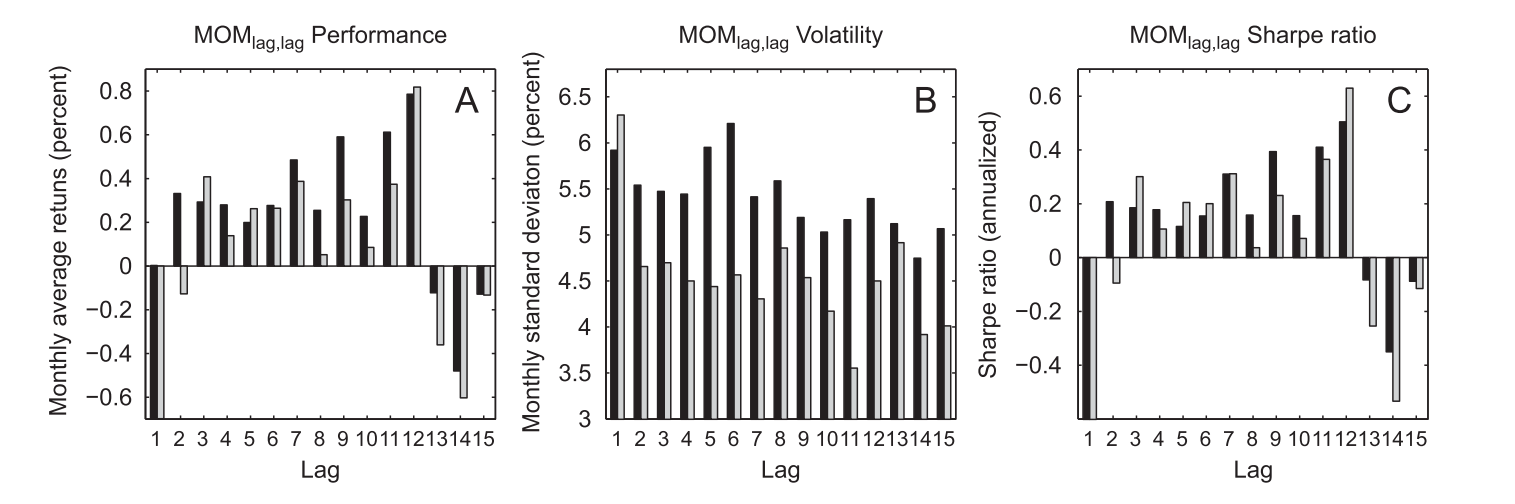
\includegraphics[width=\linewidth]{Figures/NovyMarx2012_Fig1_better.png}
  Description from original paper:
  \begin{quote}
  \textit{Fig. 1. Marginal strategy performance. This figures shows the average monthly returns (Panel A), monthly standard deviations (Panel B) and annual Sharpe ratio (Panel C) to winners-minus-losers strategies. Winners and losers are defined as the top and bottom deciles of performance in a single month, respectively, starting lag months prior to portfolio formation. Dark bars show value-weighted results and light bars show equal-weighted results. Average monthly returns for the one month reversals are $-1.04$\% (value-weighted) and $-2.82$\% (equal-weighted). The sample covers April 1927 to December 2010.}  
  \end{quote}
\end{figure}


This concept of cross-sectional momentum corresponds to the traditional idea of momentum whereas \textcite{Novy-Marx2012} finds that positive correlation is essentially coming from the first five months of the previous year, i.e. the return between $t-12$ and $t-7$ (included). The expected return and Sharpe ratio of several trading strategies tested exhibit figures twice larger for 12-to-7 winners-minus-losers (WML) portfolios compared with 6-to-2 WML portfolios. Describing a term structure of momentum put in evidence thanks to CRSP data spanning from 1926 to 2010 \textcite{Novy-Marx2012} claims that
\begin{quotation}
Theoretically, the return predictability implied by the data, which looks \emph{more like an echo than momentum}\footnote{Emphasis added in the quote.}, poses a significant difficulty for stories that purport to explain momentum.
\end{quotation}
Results in \textcite{Novy-Marx2012} indeed defeat possible and competing explanations of momentum cited in his review of literature. Nevertheless, \textcite{Goyal2015} have extensively tested and extended this surprising result: no evidence of this echo pattern has been brought outside the U.S. stock market and even in the U.S., the superior returns of 12-to-7-month sorted portfolios over their 6-to-2-month counterparts may be due to the fact that short-term reversal, usually considered over the previous month, sometimes extends further in the past over month $t-2$. I do not take any side without having tested the data from my own paper and therefore consider both alternatively in tests. The aim in this section is to explain why the momentum effect has to be included as a control in regressions involving returns or the volatility of returns, rather than provide a theoretical rationale for doing so. In general, let us summarize as follows : models ``predicting short-term predictability'' (i.e., attempting to explain momentum, as the author nuances) are in either of two categories:
\begin{description}
\item[Behavioral] Momentum arises from the delayed and progressive incorporation of news into prices, meaning that the market underreacts to a news spreading out and catches up during the following months. Thanks to a model of investor sentiment based on the famous representativeness heuristics introducted by \textcite{Tversky1974},\textcite{Barberis1998} model simultaneously underreaction in the short term (up to 12 months after news) and overreaction in the longer term, between 3 and 5 years if the stream of news is consistently good or bad, highlighting conservatism among agents. \textcite{Daniel1998} attribute momentum to what they call \emph{biased self-attribution}, which is a form of overconfidence in one's piece of privileged information and a common trait in behavioral finance \parencite{DeBondt1994}. Themselves citing another article, \textcite{Daniel1998} summarize the self-attribution bias as follows: ``Heads I win, tails it's chance.'' Confidence gets stronger, the more information confirms their private signal whereas so-called \emph{disconfirming}, i.e. contrary, evidence only reduces confidence to a little extent. Continued confirmation therefore amplifies (in intensity) and extends (over time) the agents' initial overreaction, yielding positive price auto-correlation in the short run, i.e. momentum. Both of these behavioral models assume a single representative trader whose bias causes short-lag autocorrelation in returns; \textcite{Hong1999} choose a fundamentally different approach as they segregate investors into two categories, each being ``boundedly rational'': \emph{newswatchers} are gathered into subgroups and gradually have access to private information and trade according to this piece of information but they do not condition their decision on past and current prices, only the information\footnote{The authors seem conscious of the debatable realism of their modelling regarding newswatchers, which act without observing past and present prices and thus their own previous trades. It is suggested that they act like frontrunners, taking advantage of information eearly available and conscious that their trades will start a reaction (future asset price increases in case of good news). This attitude has a limited effect in the model, which means that short term underreaction still prevails. }. \emph{Momentum traders} are the opposite category, i.e. they trade according to the price trend over a finite horizon but do not have access to any private information; in other terms, they observe, follow and extend an existing trend. Overall, in this model, the momentum effect therefore does not arise from either of the two groups of traders, rather does it appear from their interaction. While \textcite{Daniel1998} build their behavior model on psychological research results, \textcite{Barberis1998} and \textcite{Hong1999} support their models with testable hypotheses and empirical evidence.
\item[Rational] Predictions of the momentum that do not rely on investors' behavior are less frequent in literature but two contributions can be shortly summarized. First, the concern of \textcite{Johnson2002} is less about providing an equilibrium model with robust empirical evidence than show that momentum can arise even in a rational setting, along with mean-reversion approximately one-year after measurement. The fact growth rate risk rises with growth rate is at the core of the momentum effect and infrequent, persistent, e.g. technological shocks would cause most of this effect. Stocks prices depend on growth rates, because the former are modelled as a claim on a stochastic stream of dividends which grow at a random stationary rate. The growth rate risk is priced in the stock and, to quote this rather quantitative paper :
  \begin{quote}
    [M]omentum effects then follow because positive (negative) cumulative returns typically imply ex post that recent growth rate shocks have been positive (negative).
    \end{quote}
\end{description}
Another empirical paper with a real options model, \textcite{Sagi2007}, aims specifically at identiying firm-specific variables that drive momentum and thus allow to build more profitable trading strategies conditioning on those drivers, thus outperforming the baseline \textcite{Jegadeesh1993} winners-minus-losers, 6-month holding portfolio. Positive return autocorrelation due to the company value being convex in an underlying risk factor is specified in this paper, borrowing to \textcite{Johnson2002} : the underlying risk factor was the growth rate risk. Empirical findings are the following : momentum varies positively with the volatility of revenue (sales) growth, negatively with costs of goods sold and negatively with the book-to-market ratio. For the latter, it means that a more profitable momentum strategy can be implemented on firms sorted according to their book-to-market ratio; this result does not invalidate the predictive power of the book-to-market ratio over expected returns, i.e. the HML factor from \textcite{Fama1992}.

\subsubsection{Gross profitability}
\label{subsubsec:profitability}
According to \textcite{Novy-Marx2013}, gross profitability, i.e.
\begin{equation}
  \mathsf{Gross\_Profitability}_{i, t} = \frac{\mathsf{Revenues}_{i, t} - \mathsf{COGS}_{i, t}\footnotemark}{\mathsf{Total\_Assets}_{i, t}}
\end{equation}\footnotetext{Cost of goods sold}
has a prediction power equal in magnitude and complementary to the book-to-market ratio over the cross-section of expected returns. \textcite{Novy-Marx2013} has deemed this factor the \emph{other side of value} because it does not subsume it while it is linked to it. Both factors can be exploited together and improve each other's risk-adjusted performance in a portfolio. The value factor measures the market price of a company's assets and finances the purchase of inexpensive assets through the sale of expensive ones while the profitability ratio measures how productive assets within the firm are and finances the purchase of productive ones through the sale of unproductive (or at least, less productive) ones.

The influence of profitability had already been studied before \textcite{Novy-Marx2013} showed the existence of a predictive power over the cross-section of expected returns and thus the opportunity of a trading strategy : indeed \textcite{Fama2006} treat the book-to-market, profitability and investment effects combined, although the authors remain agnostic on the mechanism, either rational or behavioral, underpinning their threefold statement. The statement originates from the dividend discount model, which states that the market value of the company is equal to the sum of discounted divided expected to be paid to shareholders in the future:
\begin{equation}
  M_{t} = \sum_{\tau = 0}^{\infty}\frac{\mathbb{E}_{t}(Y_{t + \tau} - \,dB_{t + \tau})}{(1 + r)^{\tau}}
\end{equation}
where $M_{t}$ is the market value cum-dividend at time $t$; $Y_{t}$ are the earnings;$\,dB_{t} = B_{t} - B_{t - 1}$ is the increase of the book value of equity between $t - 1$ and $t$, and $r$ used in the discount factor is the required rate of return. Under the so-called clean surplus accounting, earnings are either retained within the company, thus increasing the book equity, or it is distributed to shareholders; subsequently, the difference within the expected value brackets is equal to dividends. Through this identity, \textcite{Fama2006} imply and later show that, \emph{ceteris paribus}, firms with higher earnings must yield higher expected returns (the $r$ variable) as long as their market valuations are the same, allowing the profitability premium to exist. Regarding the value premium, for fixed earnings and book value series over the whole (here, assumed infinite) time horizon, the lower the market value, the higher the expected return must be, which is gives birth to the value premium.

Overall, two measures of profitability seem to correlate with expected returns : earnings from the income statement were tested and \textcite{Fama2006} did not find an incremental predictive power beyond the size and book-to-market factors. \textcite{Novy-Marx2013} rationale for gross profitability can be summarized as follows : some expenses are treated as costs, such as R\&D, human capital development, but in fact, they will likely yield the company higher profits in the future. Therefore, one has to look at a figure higher in the income statement in order to approach the pure operating performance of the company and filter out some irrelevant costs. The same happens for the computation of free cash flows : for example, capital expenditures are not the sign that the company is less profitable, rather the opposite can be expected in the future. The author's tests putting various profitability ratios lead to conclude that gross profit over assets (and not the book equity, thus the measure is independent from the debt level) is a less-biased proxy with the most predictive power.
\subsection{Impact of ETF ownership on stocks' volatility}
\label{subsec:Method:Volatility}
The theoretical basis of all main and control variables included in the models have been discussed and the inclusion of controls is justified through a summary of the abundant literature of empirical asset pricing. In this subsection, the first identification strategy attempts to answer the question : does the share of a stock globally owned by exchange-traded funds has a contemporaneous impact over the stocks' volatility, all other characteristics being equal ? The null hypothesis being conservative (``no effect''), its potential rejection would mean that the liquidity trading hypothesis is actually reflected in the panel data with a controlled error risk level that will be disclosed in the estimation results.

Due to the structure of dataset, which is an unbalanced panel of U.S., respectively international stocks, some unique characteristics inherent to each stock will be controlled through entity fixed effects. Since the trend over the measurement period has been an exponential increase in the weight of ETFs, both in terms of stock ownership and volume traded, some fixed effects over the time axis seem legitimate. Otherwise, one could imagine that, provided that the average volatility of each stock does not significantly varies, the higher ETF ownership would results in a spuriously negative coefficient (!). Another reason for month fixed effects deals with short term market events, such as several market crashes that occurred during the two decades of the sample. 
\begin{equation}
  \mathsf{Volatility}_{i,t} = \beta_{0} + \beta_{1} \mathsf{ETF\_ownership}_{i, t} + B_{C}^{\intercal} \mathsf{Controls}_{i, t} + \alpha_{i} + \gamma_{t} + \epsilon_{i, t}
\end{equation}

Rather than a panel analysis, it would be more accurate to call this regression a dynamic panel analysis : several lags of volatility will be included among controls in some estimations in order to account for a potential case of autocorrelation in volatility. Further investigation will also control for a potential bias in the effect of the ETF ownership share over stock volatility : what if ETFs were only a symptom of the institutional ownership, which would in that case exhibit comovement with the ETF ownership. The collection of data allows us to account for certain other broad categories of institutional investors, legally forced to report their holdings: mutual funds, pension funds and hedge funds. Controlling for the aggregate ownership share of each category may help to distinguish between several channels between institutional trading and volatility.
\subsubsection{Risk of endogeneity bias : the need for an instrument}
The direct estimation of the effect of ETF ownership on volatility may bear a subtle and essential caveat: there may exist an unknown cause, an ommitted factor that would be correlated both with ETF ownership and volatility. A robust identification would alleviate this possible endogeneity bias by using an instrumental variable based on a restriction. For the instrument to be valid, it has to affect the volatility only through its correlation with ETF ownership. Since a significant share of ETFs track well-known indices, the literature (e.g. \textcite{Ben-David2018}) uses the inclusion/exclusion event of a given stock into the index to explain the variation of ETF ownership. The second step consists in an panel regression similar to the previous ones in which the observed ETF ownership is replaced with the fitted value from the first stage regression.
\subsection{Impact of ETF ownership on market and stock liquidity}
\label{subsec:Method:Liquidity}
This segment of the analysis focuses on evidence about of ETF ownership on proxies for liquidity : \textcite{Israeli2017} have shown that an increase in ETF ownership is correlated with higher trading costs, measured using the bid-ask spread, and lower liquidity, measured through a price-impact variable is equal to the numerator of \textcite{Amihud2002} ratio.

The following regression is run regarding the effect of ETF ownership on the bid-ask spread:
\begin{equation}
 \mathsf{PctBidAskSpread}_{i,t} = \beta_{0} + \beta_{1} \mathsf{ETF\_ownership}_{i, t} + B_{C}^{\intercal} \mathsf{Controls}_{i, t} + \alpha_{i} + \gamma_{t} + \epsilon_{i, t}
\end{equation}
\textcite{Israeli2017} measure this relationship in first differences using an annual panel. The stationarity concern will be investigated further and inspiration is evidently drawn from their research scheme. They add several controls and industry-level fixed effects.

The second proxy for liquidity is \textcite{Amihud2002} illiquidity ratio, which numerator and denominator may be correlated with ETF ownership : the numerator is the absolute daily return and the denominator, feared to be especially sensitive to ETF ownership's influence, is the daily dollar volume traded. A spurious improvement (lower illiquidity) could be linked with ETF ownership if the latter increases the denominator, possibly offsetting the simultaneous increase in absolute return. The proposed way to mitigate this inherent issue is to split the ratio and consider the denominator as a regressor.
\begin{equation}
   \mathsf{Illiq^{Num}}_{i,t} = \beta_{0} + \beta_{1} \mathsf{ETF\_ownership}_{i, t} + \beta_{2} \mathsf{Illiq^{Denom}} + B_{C}^{\intercal} \mathsf{Controls}_{i, t} + \alpha_{i} + \gamma_{t} + \epsilon_{i, t}
\end{equation}
\subsection{Concerns about informational efficiency}
\label{subsec:Method:Efficiency}
Pricing efficiency in \textcite{Ben-David2018} is tested as follows : they test whether the increased ETF ownership yield a higher degree of mean-reversion in pprices. In other terms, a stronger negative auto-correlation in prices (over 5 days) is the sign that they become noisier due an increased non-fundamental volatility. Such evidence is considered a empirical confirmation of the liquidity-trading hypothesis.

The variance ratio is defined as :
\begin{equation}
 VR_{i,t} = \frac{Var(r5_{i, t})}{5 \cdot Var(r1_{i, t})}
  \end{equation}

